\documentclass[11pt]{article}

\usepackage[margin=1in]{geometry}
\usepackage{amsmath,amssymb,amsfonts}
\usepackage{booktabs}
\usepackage{graphicx}
\usepackage{hyperref}
\usepackage{tikz}
\usepackage{xcolor}
\usepackage{enumitem}
\usepackage{subcaption}
\usepackage{placeins}
\usetikzlibrary{arrows.meta,positioning,fit,calc,shapes.geometric}

\title{State Is All You Need: Toward World-State Processing Units}
\author{WPU Research Prototype}
\date{\today}

\newcommand{\state}{\mathcal{S}}
\newcommand{\objects}{\mathcal{O}}
\newcommand{\relations}{\mathcal{R}}
\newcommand{\belief}{\mathcal{P}}
\newcommand{\timevar}{\mathcal{T}}
\newcommand{\deltaS}{\Delta \mathcal{S}}

\begin{document}
\maketitle

\begin{abstract}
Token sequences are a powerful substrate for language, but they are not the
natural computational primitive for persistent world processing. A world is not
only observed; it is maintained, updated, branched, corrected, and queried as
state. This paper proposes the World-State Processing Unit (WPU), a
state-native model and execution abstraction in which objects, relations, time,
uncertainty, events, and branch deltas are first-class components. The central
operation is not token attention but state propagation: events produce sparse
deltas, deltas traverse causal relations, affected regions are updated locally,
and dense recomputation is invoked only when locality breaks. We define the
token-state distinction, introduce propagation as a simplified local-physics
prior, derive a sparse-dense crossover metric, and present a small PyTorch
reference implementation, \texttt{WorldStateProcessor}. On a synthetic
robot-cup object physics task, the prototype reduces next-state prediction MSE
from 0.8111 to 0.0005 after 200 training steps and improves branch
classification accuracy from 0.1289 to 0.7188, exceeding a 0.6680 majority
baseline. Stronger v2 retrieval experiments show that explicit state also
exposes pre-propagation working-set control. A regret-distilled state retriever
wins 14 of 15 seed/K conditions against an interaction-teacher retriever, and a
newer cross-seed experiment shows that risk-adjusted mechanism selection over
state-native role/geometry/family descriptors improves held-out loss over a
static learned selector for \(K=8,16,32\) at \(N=2048\). These results do not
establish broad world understanding. They establish a falsifiable research
program: if world
processing is dominated by persistent identity, local causal change,
uncertainty, branching, and small event-conditioned causal working sets, then
state should be treated as a primary computational substrate rather than as a
serialization target for tokens. The experimental objective is to map the
regime where this substrate is useful, not to claim universal superiority over
token, graph, or latent world models.
\end{abstract}

\section{Introduction}

The dominant abstraction in modern deep learning is the token sequence. A token
sequence is a list of symbols or embeddings processed through position-indexed
operations, most notably attention. This abstraction has been remarkably
successful for language and for many domains that can be serialized into a
sequence. However, world processing has a different structure. Physical and
simulated worlds contain persistent objects, typed relations, heterogeneous
attributes, temporal continuity, uncertainty, local causal effects, and multiple
possible futures.

This paper asks a narrow question: if the target workload is world processing,
should the fundamental unit be the token or the state? We argue that tokens can
\emph{describe} state, but they do not preserve state as a computational
invariant. A cup can be serialized into text, but the resulting sequence does
not make object identity, relation locality, delta updates, uncertainty, or
branch sharing first-class operations. A state-native model should not merely
retrieve relevant positions; it should update persistent entities and propagate
the consequences through a structured world memory.

We call the required conversion \emph{objectification}: an observation,
simulator export, database state, or tracker output is converted into
persistent, addressable objects with typed attributes, role/affordance state,
typed relations, uncertainty, admissible deltas, and branch-local overlays.
Objectification is not a claim that perception is solved; it is the contract that defines the
state substrate consumed by WPU. The reference implementation treats this as a
measurable contract rather than a slogan: identity coverage, relation endpoint
validity, confidence, delta validity, and causal-working-set locality can be
reported before propagation. This separates a WPU failure caused by poor
objectification from a failure caused by the propagation model itself. In the
current scheduler, the same contract can act as a safety signal: low
objectification quality escalates execution away from blind sparse propagation
toward hybrid or dense recomputation.
If object identity exists but local relation extraction misses an edge, the
prototype can add conservative geometry-derived relation-repair patches. These
patches are treated as hypotheses for frontier recovery, not as discovered
physical laws. The repair probe now separates nominal type labels from
relation-bearing object state. Ungated geometry repair recovers frontier recall
but attaches distractors, and the precision collapse worsens under denser
distractors. Hand-written type gating preserves precision only while type names
match the gate. A small learned scorer transfers across aliased type names when
role/affordance variables are preserved, but fails when both type and role
information are removed. This makes the objectification boundary falsifiable:
WPU does not need names alone; it needs persistent state variables that can
support relation hypotheses. A toy downstream diagnostic closes the first
repair-to-prediction loop: role-aware learned repair improves aliased-type
branch accuracy from 0.343750 to 0.671875 and lowers loss from 1.319667 to
0.885275, while ungated dense-distractor repair restores frontier recall but
worsens loss.
A second toy probe tests whether relation candidates can be learned from object
histories and transferred to a held-out mechanism family. A history scorer
trained on \texttt{contact\_transfer} and \texttt{support\_transfer} reaches
five-seed mean relation precision/recall 0.987500 on held-out
\texttt{hidden\_field}, improving downstream accuracy from 0.494531 to
0.992188. This is still synthetic evidence; it is not a claim of physical-law
discovery.
A third toy probe tests relation-to-law transfer. A history-derived relation
selector plus an interpretable inverse-distance local law transfers to renamed
held-out \texttt{hidden\_inverse}, reaching five-seed mean relation
precision/recall 0.988281 and delta MSE 0.000828 versus 0.445909 for no relation
or type prior. This is a controlled synthetic bridge from objectification to
approximate local theory, not evidence of unknown-law discovery.
An OOD version maps the failure boundary: the relation/law stack remains useful
under distance, gain, and denominator shifts, but far-distance relation recall
drops to 0.658594, and shifted gain or law form leaves residual MSE even with
oracle relations. Thus the intended WPU loop is not ``fit a law once''; it is
objectify, propose a local rule, stress it, and revise the rule when OOD error
separates relation failure from law mis-specification.
A revision probe shows this loop can be made operational in the synthetic
setting. With 64 calibration samples, gain calibration reduces
\texttt{hidden\_inverse\_gain\_shift} MSE from 0.115978 to 0.000342; form
revision reduces \texttt{hidden\_power\_shift} MSE from 0.054596 to 0.008887.
Oracle-relation form revision reaches 0.000232, identifying the remaining gap as
relation selection and calibration noise rather than only law-form capacity.
The implementation exposes this loop as reporting primitives:
\texttt{LocalLawHypothesis} stores an interpretable rule candidate, and
\texttt{LawRevisionReport} records base/revised error, revision decision, and
optional relation-selection versus law-residual attribution.

We introduce the World-State Processing Unit (WPU) as both a model family and an
execution abstraction. It is not proposed as a replacement for GPUs, TPUs, or
NPUs as general numerical accelerators. Instead, it is a workload definition for
world-state processing: a WPU maintains explicit state memory, performs sparse
event-driven propagation when changes are local, falls back to dense recompute
when affected regions become large, and represents alternative futures as
deltas over a shared base state.

\paragraph{Central thesis.}
The central thesis is that world processing is not primarily a problem of
continuing a sequence; it is a problem of maintaining a changing state under
partial observation. Tokens are excellent carriers of evidence, but state is the
substrate on which consequences accumulate. A state-native model should
therefore make identity, locality, delta update, uncertainty, and branching
operationally explicit.

\paragraph{Contributions.}
This paper makes four contributions. First, it formulates a token-state
non-equivalence claim in operational rather than representational terms: tokens
can serialize state, but serialization does not preserve state operations as
invariants. Second, it defines objectification as the construction of persistent
state objects, makes objectification quality measurable as a pre-propagation
contract, and treats propagation as the central operation over object
relations, relating this to simplified local physical causality.
Third, it proposes a WPU architecture with sparse, hybrid, and dense execution
paths selected by an affected-state crossover metric. Fourth, it provides a
minimal reference implementation and small-scale validation task, intended as a
starting point for stronger benchmarks rather than as final evidence.

\begin{figure}[t]
\centering
\resizebox{0.98\linewidth}{!}{%
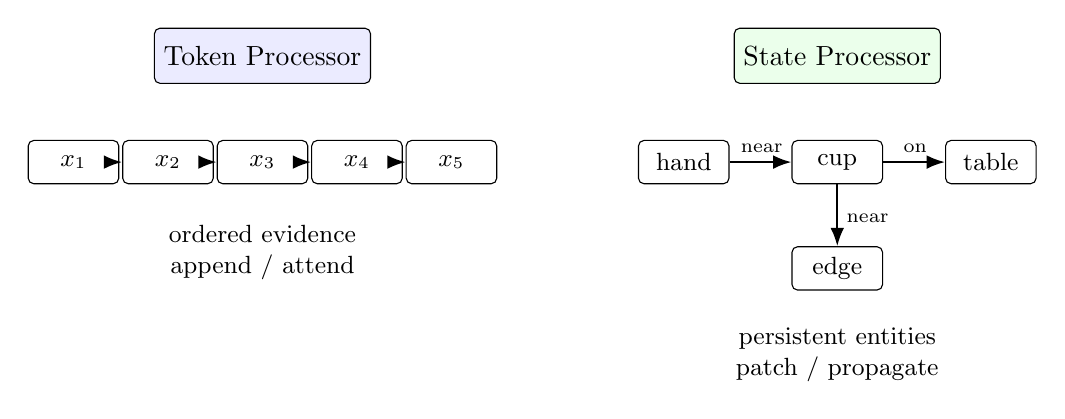
\begin{tikzpicture}[
  box/.style={draw, rounded corners=2pt, minimum width=2.0cm, minimum height=0.7cm, align=center},
  small/.style={draw, rounded corners=2pt, minimum width=1.15cm, minimum height=0.55cm, align=center, font=\small},
  arrow/.style={-Latex, thick}
]
\node[box, fill=blue!8] (toktitle) at (0,1.35) {Token Processor};
\node[small] (t1) at (-2.4,0) {$x_1$};
\node[small] (t2) at (-1.2,0) {$x_2$};
\node[small] (t3) at (0,0) {$x_3$};
\node[small] (t4) at (1.2,0) {$x_4$};
\node[small] (t5) at (2.4,0) {$x_5$};
\draw[arrow] (t1) -- (t2);
\draw[arrow] (t2) -- (t3);
\draw[arrow] (t3) -- (t4);
\draw[arrow] (t4) -- (t5);
\node[align=center, font=\small] (tokcap) at (0,-1.15) {ordered evidence\\append / attend};

\node[box, fill=green!8] (statetitle) at (7.3,1.35) {State Processor};
\node[small] (cup) at (7.3,0) {cup};
\node[small] (hand) at (5.35,0) {hand};
\node[small] (table) at (9.25,0) {table};
\node[small] (edge) at (7.3,-1.35) {edge};
\draw[arrow] (hand) -- node[above, pos=0.52, yshift=2pt, font=\scriptsize, fill=white, inner sep=1pt] {near} (cup);
\draw[arrow] (cup) -- node[above, pos=0.52, yshift=2pt, font=\scriptsize, fill=white, inner sep=1pt] {on} (table);
\draw[arrow] (cup) -- node[right, pos=0.55, xshift=2pt, font=\scriptsize, fill=white, inner sep=1pt] {near} (edge);
\node[align=center, font=\small] at (7.3,-2.45) {persistent entities\\patch / propagate};
\end{tikzpicture}
}
\caption{Token processing operates over ordered evidence. State processing
operates over persistent entities and relations. The distinction is not what can
be represented, but which operations are first-class.}
\label{fig:token-state}
\end{figure}

\section{Relation to Existing Work}

WPU is deliberately positioned near several mature research lines rather than
outside them. Object-centric representation learning studies how objects can be
discovered from perceptual input, including iterative variational inference and
slot-based attention mechanisms \cite{greff2019iodine,locatello2020slot}. Graph
networks and interaction networks show that object- and relation-centric message
passing is a powerful inductive bias for physical reasoning
\cite{battaglia2016interaction,battaglia2018relational,sanchezgonzalez2020gns}.
Set Transformers and Graph Transformers show how attention can be adapted to
sets and graphs \cite{lee2019set}. Latent world-model agents such as PlaNet,
Dreamer, DreamerV3, and IRIS learn compact dynamics models for planning or
imagination \cite{hafner2019planet,hafner2020dreamer,hafner2023dreamerv3,micheli2022iris}.
Recent object-centric and graph world models further emphasize structured
entities, causal interactions, sparse attention, and planning over object
representations
\cite{nishimoto2026stica,vakhitov2026objectzero,lei2025spartan,liu2026graphworldmodels}.

The WPU claim is therefore not that message passing, object-centric modeling, or
world models are new. The distinction is operational and systems-oriented. WPU
treats persistent state, event frontiers, sparse-dense routing, delta overlays,
branch sharing, and update work as the primary interface. In contrast, most
prior world models define a learned dynamics model and then optimize control or
prediction quality; most object-centric perception models focus on extracting
objects; most graph simulators focus on accurate dynamics under a chosen graph;
and most sparse Transformer models keep attention as the central operation. WPU
asks a different question: what execution abstraction is appropriate when the
workload is maintaining and branching a large world state under local events?

This also clarifies an important limitation. The current prototype assumes that
the object-relation state is already available. A complete WPU system would need
a perception front-end, such as slot/object discovery or supervised
segmentation, to construct and repair the state graph from pixels, point clouds,
or multimodal observations. This front-end is outside v1 and is treated as a
required next step, not as a solved problem. In the near term, perception should
be treated as an object-state adapter layer: WPU can consume state graphs from
supervised detectors, object discovery modules, simulators, or logs while the
core execution question remains focused on update work, prediction risk, and
branch memory.

\section{Token and State Primitives}

\subsection{Token}

A token model receives a sequence
\[
X = (x_1, x_2, \ldots, x_T), \quad x_t \in \mathbb{R}^d.
\]
Its memory is usually position-indexed: sequence context, hidden activations, or
KV cache. The central operation in a Transformer is attention:
\[
\mathrm{Attn}(Q,K,V)=\mathrm{softmax}\left(\frac{QK^\top}{\sqrt{d}}\right)V.
\]
This operation answers: which positions should a position retrieve from?

\subsection{State}

A world state is a persistent structured object:
\[
\state_t = \{\objects_t, \relations_t, \timevar_t, \belief_t\}.
\]
Here \(\objects_t\) is a set of object records, \(\relations_t\) is a typed
relation graph, \(\timevar_t\) is temporal memory, and \(\belief_t\) represents
uncertainty. An event \(e_t\) produces a delta:
\[
\state_{t+1} = \state_t \oplus \deltaS_t.
\]
The central operation is propagation:
\[
\delta o_i^{(\ell+1)} =
f_\theta\left(o_i, e_t, \sum_{j \in \mathcal{N}(i)}
g_\theta(o_i, r_{ij}, o_j, \delta o_j^{(\ell)})\right).
\]
This operation answers: what changed, which objects are causally affected, and
how far should the consequences propagate?

Propagation is also a deliberately simplified physical prior. Many useful
physical approximations are local: contact forces, support constraints,
occlusion, collision risk, and signal flow usually begin at a small set of
entities and spread through nearby relations. The WPU does not claim that this
local propagation is exact physics. It claims that, for many world-processing
regimes, local causal propagation can play the role that simplified Newtonian
mechanics plays below relativistic scales: an approximate but operationally
useful computation before a more global correction is needed.

\subsection{Non-equivalence Claim}

The claim is not that tokens cannot encode state. Any finite state can be
serialized. The claim is that serialization does not preserve the operational
invariants needed for efficient world processing: persistent identity, local
delta update, relation-addressed propagation, branch sharing, and uncertainty
updates. In short:
\[
\text{Token} = \text{representation of evidence}, \quad
\text{State} = \text{substrate of update}.
\]

This distinction is important because representational universality can obscure
computational mismatch. A text string can describe a database, a graph, or a
physical scene, but the string does not by itself provide indexed update,
referential integrity, graph traversal, or copy-on-write branching. The WPU
proposal is analogous: it does not deny that token models can learn world
regularities; it claims that world-state operations should not have to be
reconstructed from sequence position at every step.

\begin{table}[t]
\centering
\begin{tabular}{lll}
\toprule
Property & Token sequence & World state \\
\midrule
Basic unit & position embedding & object / relation / belief \\
Identity & implicit in context & explicit object identity \\
Memory update & append or rewrite & patch existing state \\
Relation & inferred by attention & stored as typed edge \\
Future & continuation & branch overlay \\
Typical target & next token & next state / delta / branch \\
\bottomrule
\end{tabular}
\caption{Token and state differ at the level of computational primitive, not
merely at the level of data format.}
\label{tab:token-state}
\end{table}

\section{Why a WPU?}

GPUs, TPUs, and NPUs are excellent dense numerical engines. LPUs and similar
sequence-oriented systems emphasize token streams. A WPU is defined by a
different workload: world-state maintenance and update.

This workload has four recurring properties. First, most state persists across
time. Second, most events affect only a small subset of the state. Third,
effects propagate through a structured neighborhood rather than uniformly across
all entities. Fourth, future uncertainty is often branching: multiple
hypotheses share the same past and differ only in local deltas. A processor that
treats all state as a fresh dense input at every step ignores these properties.

The term ``processing unit'' is used here as a workload and execution-abstraction
claim, not as a completed chip design. Recent accelerator proposals for language
or reasoning inference emphasize memory bandwidth and token-generation
bottlenecks \cite{adiletta2026rpu}, while neuromorphic and sparse-computation
surveys emphasize event-like sparsity and recurrent state dynamics
\cite{simeone2026neuromorphic}. WPU is complementary: it identifies the memory
objects and update operations that a future world-state accelerator would need,
but the present implementation remains a PyTorch reference model. Hardware,
chiplet, or edge-processor claims should therefore be read as future hypotheses,
not as conclusions of this paper.

The performance claim is conditional. If the world has \(N\) objects, an event
initially changes \(\Delta N\) objects, relation fanout is \(k\), propagation
depth is \(h\), and there are \(B\) branches, then the affected fraction is
\[
\rho = \frac{\Delta N k^h B}{N}.
\]
Dense recomputation is roughly \(O(N)\) for set-level processing or \(O(N^2)\)
for full attention. Sparse WPU propagation is approximately
\[
O(\Delta N k^h B).
\]
Therefore, when \(\rho \ll 1\), sparse state propagation can be more efficient
than full dense recomputation. When \(\rho\) is large, the WPU should route to
hybrid or dense computation. The WPU advantage is not universal; it is
workload-dependent and measurable.

This complexity model is intentionally incomplete as a hardware model. It does
not include graph construction, dynamic edge repair, irregular memory access,
frontier queue overhead, scatter/gather efficiency, kernel launch overhead, or
state-corruption recovery. Those terms determine whether a WPU-style design
actually outperforms dense accelerators on real hardware. The v1 experiments
therefore report CPU latency and work proxies, but they should not be read as
final hardware evidence. A software runtime or middleware layer is the nearer
term target: only after measuring frontier queues, relation fetch, scatter/gather,
sparse kernels, delta logs, branch-overlay memory, and recovery costs can a
hardware target be specified responsibly.

\paragraph{Conditional performance proposition.}
For workloads in which \(\Delta N k^h B \ll N\), a WPU-style update has lower
asymptotic state-update work than dense recomputation while preserving access to
dense correction when locality fails. For workloads in which the affected
region is global, the WPU should reduce to dense computation and offers no
sparse advantage. This conditional nature is a feature of the proposal: it makes
the claim measurable and falsifiable.

\section{WPU Architecture}

\begin{figure}[t]
\centering
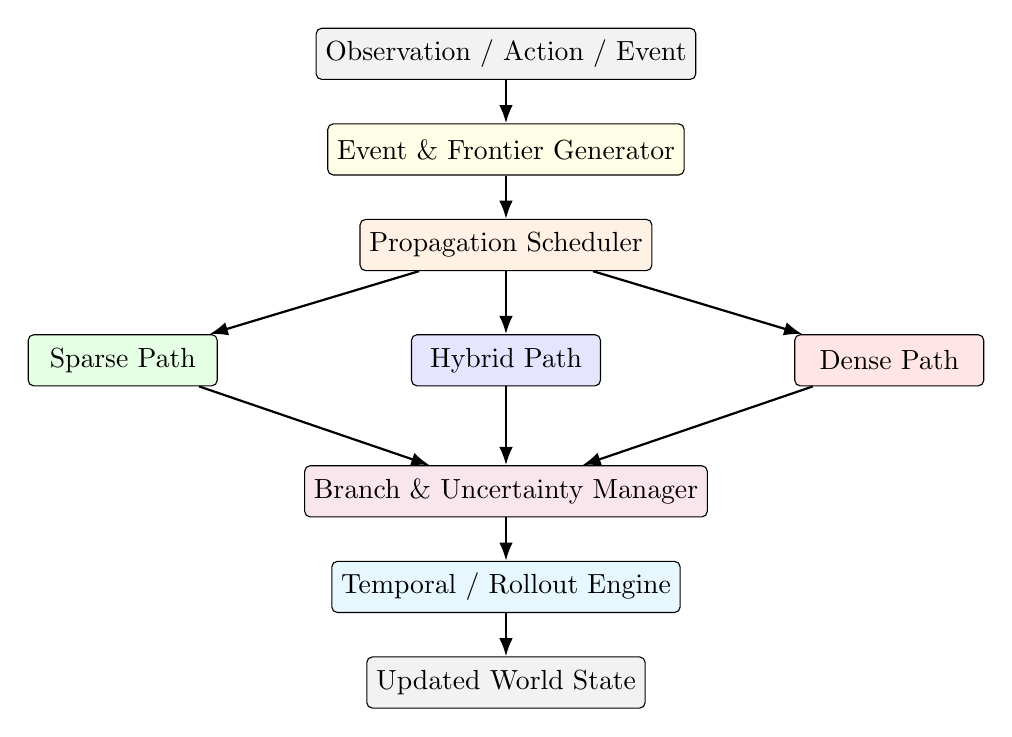
\begin{tikzpicture}[
  node distance=0.55cm,
  block/.style={draw, rounded corners=2pt, minimum width=2.8cm, minimum height=0.65cm, align=center},
  pathblock/.style={draw, rounded corners=2pt, minimum width=2.4cm, minimum height=0.65cm, align=center},
  arrow/.style={-Latex, thick}
]
\node[block, fill=gray!10] (event) {Observation / Action / Event};
\node[block, below=of event, fill=yellow!10] (frontier) {Event \& Frontier Generator};
\node[block, below=of frontier, fill=orange!10] (sched) {Propagation Scheduler};
\node[pathblock, below left=0.8cm and 1.8cm of sched, fill=green!10] (sparse) {Sparse Path};
\node[pathblock, below=0.8cm of sched, fill=blue!10] (hybrid) {Hybrid Path};
\node[pathblock, below right=0.8cm and 1.8cm of sched, fill=red!10] (dense) {Dense Path};
\node[block, below=1.0cm of hybrid, fill=purple!10] (branch) {Branch \& Uncertainty Manager};
\node[block, below=of branch, fill=cyan!10] (rollout) {Temporal / Rollout Engine};
\node[block, below=of rollout, fill=gray!10] (state) {Updated World State};
\draw[arrow] (event) -- (frontier);
\draw[arrow] (frontier) -- (sched);
\draw[arrow] (sched) -- (sparse);
\draw[arrow] (sched) -- (hybrid);
\draw[arrow] (sched) -- (dense);
\draw[arrow] (sparse) -- (branch);
\draw[arrow] (hybrid) -- (branch);
\draw[arrow] (dense) -- (branch);
\draw[arrow] (branch) -- (rollout);
\draw[arrow] (rollout) -- (state);
\end{tikzpicture}
\caption{WPU schematic. Events generate frontiers, the scheduler chooses a
sparse, hybrid, or dense execution path, and branches are maintained as deltas
over shared state.}
\label{fig:wpu-architecture}
\end{figure}

A WPU has five components:

\begin{enumerate}[leftmargin=*]
\item \textbf{State memory}: object store, relation graph, temporal buffer,
belief store, and branch delta store.
\item \textbf{Frontier generator}: maps observations and actions to initially
changed objects.
\item \textbf{Propagation core}: performs event-conditioned sparse message
passing through typed relations.
\item \textbf{Dense fallback}: performs global or regional recomputation when
the affected fraction is high.
\item \textbf{Branch manager}: maintains multiple futures as deltas rather than
full state copies.
\end{enumerate}

\paragraph{Memory model.}
The memory hierarchy is not an implementation detail; it is part of the
computational claim. Token systems primarily cache sequence positions. A WPU
caches persistent objects, typed relations, recent deltas, uncertainty, and
branch overlays. The intended memory operations are lookup-by-identity,
neighbor-fetch, delta-append, branch-overlay, and region materialization.

\section{Propagation Rather Than Attention}

Attention remains useful inside a WPU, especially for dense fallback and global
consistency. The claim is not that attention is obsolete. The claim is that
attention is not the defining operation for world-state processing. For token
models, attention retrieves information across positions. For WPU models,
propagation computes consequences across causal relations.

This gives propagation a physical interpretation. In the same way that a
mechanical disturbance first affects objects in contact or support relation, a
state delta should first update the frontier of causally adjacent entities. The
dense path is then analogous to a global correction step: it is invoked when the
local approximation is no longer sufficient because the affected region has
become too large.

The analogy is not that WPU propagation is a complete physical law. The analogy
is methodological. Newtonian mechanics remains useful in regimes where
relativistic corrections are negligible because it captures a stable low-order
structure of the world. Similarly, local propagation is proposed as a low-order
computational prior for many world-processing regimes: useful where causal
effects are local, insufficient where long-range coupling dominates, and
therefore paired with a dense correction path.

\begin{figure}[t]
\centering
\resizebox{0.78\linewidth}{!}{%
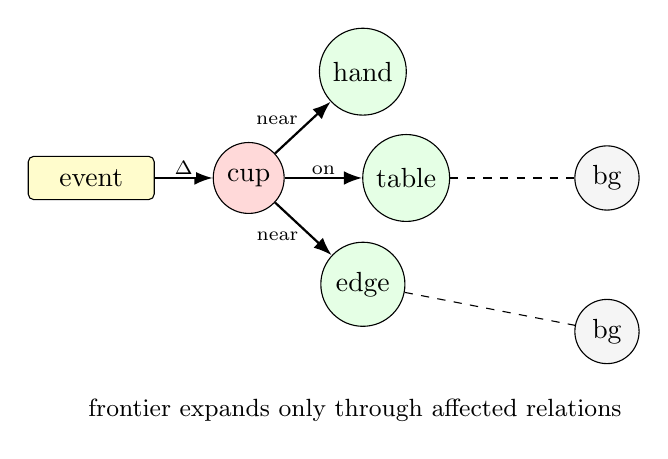
\begin{tikzpicture}[
  obj/.style={circle, draw, minimum size=0.76cm, align=center},
  event/.style={draw, rounded corners=2pt, fill=yellow!20, minimum width=1.6cm, minimum height=0.55cm},
  arrow/.style={-Latex, thick},
  edgelabel/.style={font=\scriptsize, fill=white, inner sep=1pt}
]
\node[event] (evt) at (0,0) {event};
\node[obj, fill=red!15] (cup) at (2.0,0) {cup};
\node[obj, fill=green!10] (hand) at (3.45,1.35) {hand};
\node[obj, fill=green!10] (table) at (4.0,0) {table};
\node[obj, fill=green!10] (edge) at (3.45,-1.35) {edge};
\node[obj, fill=gray!8] (bg1) at (6.55,0) {bg};
\node[obj, fill=gray!8] (bg2) at (6.55,-1.95) {bg};
\draw[arrow] (evt) -- node[above, edgelabel] {$\Delta$} (cup);
\draw[arrow] (cup) -- node[pos=0.48, above left, edgelabel] {near} (hand);
\draw[arrow] (cup) -- node[above, edgelabel] {on} (table);
\draw[arrow] (cup) -- node[pos=0.48, below left, edgelabel] {near} (edge);
\draw[dashed] (table) -- (bg1);
\draw[dashed] (edge) -- (bg2);
\node[align=center, font=\small] at (3.35,-2.95) {frontier expands only through affected relations};
\end{tikzpicture}
}
\caption{State propagation. An event produces a delta at a target object, and
the delta propagates through typed relations until the scheduler stops or
escalates the update.}
\label{fig:propagation}
\end{figure}

\section{Reference Implementation}

We implemented a small PyTorch reference model named
\texttt{WorldStateProcessor}. It receives a \texttt{StateGraphBatch} containing
object features, relation indices, relation features, event features, masks, and
scheduler metrics. It predicts object deltas, relation logits, uncertainty, and
branch probabilities.

The prototype has three paths:
\begin{itemize}[leftmargin=*]
\item \textbf{Sparse}: learned relation-conditioned message passing from the
event target.
\item \textbf{Hybrid}: sparse update plus regional dense correction.
\item \textbf{Dense}: global attention over the object set.
\end{itemize}

The scheduler uses fixed thresholds:
\[
\rho < 0.05 \rightarrow \text{sparse}, \quad
\rho < 0.25 \rightarrow \text{hybrid}, \quad
\rho \geq 0.25 \rightarrow \text{dense}.
\]

These thresholds are engineering defaults for making the v1 route behavior
inspectable. They are not claimed to be optimal constants. The supplementary
\(B\)-sweep and training-step sweep show that fixed thresholds can hurt
accuracy; in this paper, the hard scheduler is evidence for a routing
hypothesis, not a final routing policy.

The v2 scheduler should therefore optimize prediction risk and update cost
jointly. It should be able to choose regional dense correction even when
\(\rho\) is small, or sparse propagation in large worlds, when uncertainty,
fanout, relation quality, or branch divergence make that route preferable.

The reference implementation is intentionally small. It should be read as an
executable specification of the architecture, not as an optimized model. The
important interface is that the same module consumes structured state graphs,
routes computation by affected-state metrics, predicts deltas instead of only
labels, and emits branch probabilities that can be stored as overlays.

\section{Small-Scale Validation}

\begin{figure}[t]
\centering
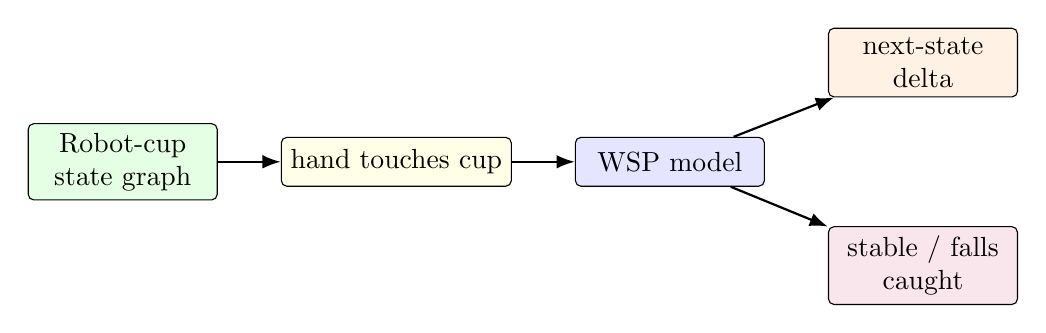
\begin{tikzpicture}[
  node distance=0.6cm,
  block/.style={draw, rounded corners=2pt, minimum width=2.4cm, minimum height=0.62cm, align=center},
  arrow/.style={-Latex, thick}
]
\node[block, fill=green!10] (scene) {Robot-cup\\state graph};
\node[block, right=0.8cm of scene, fill=yellow!10] (event) {hand touches cup};
\node[block, right=0.8cm of event, fill=blue!10] (model) {WSP model};
\node[block, above right=0.5cm and 0.8cm of model, fill=orange!10] (delta) {next-state\\delta};
\node[block, below right=0.5cm and 0.8cm of model, fill=purple!10] (branch) {stable / falls\\caught};
\draw[arrow] (scene) -- (event);
\draw[arrow] (event) -- (model);
\draw[arrow] (model) -- (delta);
\draw[arrow] (model) -- (branch);
\end{tikzpicture}
\caption{Validation task. The model observes an object-relation state graph and
an event, then predicts next-state deltas and future branch probabilities.}
\label{fig:validation}
\end{figure}

The validation task is a synthetic robot-cup object physics problem. The scene
contains a cup, table, robot hand, table edge, and configurable background
objects. The event is a hand touching the cup with variable force. The model
predicts the next object delta and one of three branch labels: stable, falls, or
caught.

This task is deliberately not a benchmark of general physical reasoning. It is
a unit test for the WPU hypothesis: can an explicit state graph, a local event,
a sparse-dense route decision, and branch probabilities be trained and inspected
in a single neural model? The experiment is therefore closer to a controlled
physics-inspired assay than to a claim of broad physical competence.

\begin{table}[t]
\centering
\begin{tabular}{lccc}
\toprule
Model & Next-state MSE & Branch NLL & Branch accuracy \\
\midrule
Untrained WSP & 0.8111 & 1.2070 & 0.1289 \\
Majority baseline & -- & -- & 0.6680 \\
Trained WSP & 0.0005 & 0.8074 & 0.7188 \\
\bottomrule
\end{tabular}
\caption{Small-scale validation on 256 synthetic evaluation samples. The model
was trained for 200 steps with batch size 16.}
\label{tab:results}
\end{table}

\begin{figure}[t]
\centering
\begin{subfigure}{0.98\linewidth}
\centering

\includegraphics[width=0.95\linewidth]{docs/figures/route_regime.png}
\caption{Routed WPU execution-path ratios as world size and branch pressure
vary.}
\end{subfigure}

\begin{subfigure}{0.98\linewidth}
\centering

\includegraphics[width=0.72\linewidth]{docs/figures/accuracy_work_tradeoff.png}
\caption{Accuracy and routed work versus world size at \(B=3\), aggregated over
seeds.}
\end{subfigure}
\caption{Regime evidence. The route diagram supports the WPU scheduler
hypothesis, while the accuracy/work plot shows that lower routed work and higher
accuracy do not automatically occur in the same \(N\) regime.}
\label{fig:regime-results}
\end{figure}

\begin{figure}[t]
\centering
\begin{subfigure}{0.98\linewidth}
\centering

\includegraphics[width=0.95\linewidth]{docs/figures/robust_accuracy_ci.png}
\caption{Accuracy with 95\% confidence intervals over five seeds.}
\end{subfigure}

\begin{subfigure}{0.98\linewidth}
\centering

\includegraphics[width=0.95\linewidth]{docs/figures/robust_accuracy_runtime.png}
\caption{Accuracy-runtime surface at branch pressure \(B=3\).}
\end{subfigure}
\caption{Robust evidence package. WPU variants are strongest in the medium
local synthetic regimes, but graph/token baselines dominate accuracy at
\(N=204\). Runtime advantage appears only at large \(N\), where the current WPU
accuracy fails.}
\label{fig:robust-results}
\end{figure}

\FloatBarrier

\section{V2 Retrieval: Risk-Adjusted Working-Set Control}

The v1 experiments identify a precise failure boundary: sparse routed work can
become attractive before sparse WPU accuracy remains reliable. The v2 question
is therefore not only how to propagate better, but how to choose the local
working set that should be propagated and which retrieval mechanism should be
deployed. This is where explicit state creates an additional intervention
point. Before any tensor propagation step, the system can select objects from
the event frontier, score alternative working sets, and train that selection
policy against downstream state-prediction regret.

Earlier learned retrievers imitated a hand-built interaction-density selector.
That objective is state-native, but it optimizes teacher overlap rather than
branch prediction loss. The retriever-regret oracle probe showed that the
interaction selector is rarely the downstream oracle. We therefore first
evaluated a regret-distilled retriever. On a validation split, the system evaluates base
candidates \(\{\texttt{indexed}, \texttt{proximity}, \texttt{interaction},
\texttt{learned}\}\) and generated local candidates. For each sample, the
candidate set with the lowest downstream branch cross-entropy is treated as a
pseudo-label object set. A small state-native object scorer is then trained to
recover that set from object/event features.

\begin{table}[t]
\centering
\begin{tabular}{lcccc}
\toprule
\(K\) & Learned-interaction loss & Regret-distilled loss & Accuracy before & Accuracy after \\
\midrule
8 & 0.988727 & 0.977017 & 0.508889 & 0.542222 \\
16 & 0.966098 & 0.955077 & 0.504444 & 0.513333 \\
32 & 1.004100 & 0.999112 & 0.480000 & 0.513333 \\
\bottomrule
\end{tabular}
\caption{Regret-distilled retrieval at \(N=2048\), averaged over five seeds.
The regret-distilled retriever is trained from validation candidate sets that
minimize downstream branch loss, rather than from the hand-built interaction
teacher.}
\label{tab:regret-distillation}
\end{table}

The regret-distilled retriever improves downstream loss at every tested \(K\)
on average and wins 14 of 15 seed/K conditions against the learned interaction
retriever. It also changes working-set composition: it selects fewer obstacles
and does not always force the hand into the working set, more closely matching
the generated oracle than the interaction teacher under the current budget.

This result strengthens the WPU claim in a specific way. Explicit state is
useful not only because it enables sparse propagation; it also exposes
object-level working-set control as a trainable pre-propagation operation.
Token baselines can serialize the same scene, but they do not naturally expose
this object-level intervention point as an independent control surface.

The same-seed result is not sufficient as a cross-seed claim. We therefore
tested a stricter mechanism-selection variant. Candidate sets are described by
explicit state-native features: hand inclusion, selected obstacle ratio,
obstacle pair density, event force, event-relative obstacle distance
statistics, lateral spread, target-axis alignment, hand/edge distance, and
candidate-family flags. The deployed policy selects among static learned
interaction, composition-aware candidates, and an invariant set scorer using
train-seed evidence. A strict no-harm seed-stable gate is too conservative at
\(K=32\); a risk-adjusted selector, which penalizes worst-seed harm without
requiring zero harm on every training seed, gives the best deployed tradeoff.

\begin{table}[t]
\centering
\begin{tabular}{lcccc}
\toprule
\(K\) & Static learned loss & Risk-adjusted loss & Accuracy before & Accuracy after \\
\midrule
8 & 0.988432 & 0.982002 & 0.506667 & 0.522222 \\
16 & 0.966183 & 0.951243 & 0.504444 & 0.517778 \\
32 & 1.004095 & 1.002597 & 0.475556 & 0.522222 \\
\bottomrule
\end{tabular}
\caption{Risk-adjusted state-native mechanism selection at \(N=2048\),
averaged over five held-out seeds. Candidate mechanisms are selected from
train-seed evidence using explicit role/geometry/family descriptors before
propagation.}
\label{tab:risk-adjusted-selection}
\end{table}

This result sharpens the WPU claim further. Explicit state is useful not only
because it enables sparse propagation; it also exposes object-level working-set
control and mechanism routing as trainable pre-propagation operations. Token
baselines can serialize the same scene, but they do not naturally expose this
object-level intervention point as an independent control surface.

The result remains bounded. Opaque set evaluators, score-margin confidence
gates, strict no-harm seed-stable gates, and cross-fit ensemble regret gates do
not solve the cross-seed selection problem, and the candidate oracle remains
substantially better. In the latest cross-fit probe, best closure falls to
0.287268 and cross-fit selected closure to 0.270989, below direct
candidate-regret gating. Descriptor standardization plus group-DRO no-harm
training is also insufficient as a detached selector: best closure is 0.110889
and train-selected closure is 0.093863. The unresolved v2 problem is therefore
candidate scoring learned jointly with retrieval and propagation, not merely
the generation of more candidate sets or post-hoc deployment gates.

A separate PyBullet branch-prior audit adds an important boundary to the shift
claim. In the \texttt{catch\_heavy} mechanism, the majority branch prior reaches
0.753968 accuracy, while the best WPU model reaches 0.408730. Thus this regime
is not a clean propagation success even when WPU beats other learned baselines;
it is a prior-adaptation failure. Mechanism-aware branch priors and
uncertainty-gated recompute are therefore required v2 components rather than
optional calibration refinements. A small seven-seed mechanism-prior adaptation
probe raises shifted WPU win-rate to 0.666667, but worsens mean shifted WPU ECE
by 0.024819. A prior-strength sweep finds an accuracy-best nonzero strength
(0.75), but no nonzero strength preserves or improves win-rate relative to
zero strength without increasing ECE. Calibration-safe prior adaptation
therefore remains open. A calibration-selected prior follow-up improves shifted
mean WPU ECE by -0.046204 and Brier by -0.105470, but leaves shifted
WPU-versus-baseline win-rate at 0.333333. Thus branch-probability calibration
and robust mechanism generalization must be reported separately. A few-shot
mechanism adaptation follow-up reaches shifted WPU-versus-baseline win-rate
1.000000 and mean margin change 0.050264, but uses mechanism-specific
calibration samples. It is evidence for an adapted regime, not for zero-shot
physical generalization. A mechanism-aware adaptive policy strengthens this
adapted regime by using selected-prior adaptation for high prior-shift cases
and few-shot parameter adaptation otherwise: shifted win-rate remains 1.000000,
mean accuracy changes by 0.198412, margin by 0.058201, ECE by -0.099347, and
Brier by -0.155443. This is detect-and-adapt evidence, not zero-shot evidence.
A separate 7-seed composition-shift stress probe is a
stronger zero-shot positive sub-regime: WPU local-dense wins all three compound
mechanisms with mean accuracy delta 0.071428, but mean ECE ratio is 1.014879,
so accuracy and calibration remain separate claims.
We also ran a WPU-only uncertainty-gated recompute probe on the same compound
shift family. Routing low-confidence sparse predictions to the WPU local-dense
path improves aggregate accuracy by 0.071428 and ECE by -0.016396, but the
effective dense recompute rate is 0.985450. A low-cost threshold with recompute
rate 0.025132 improves accuracy by only 0.009260 and worsens ECE by 0.005395.
This is a useful negative constraint: uncertainty routing is a plausible WPU
control surface, but static confidence thresholds do not yet provide a
low-cost calibrated policy.
A learned sparse-output benefit gate narrows the constraint further. Using only
sparse branch probabilities, entropy/margin, and event features, a source-trained
low-cost gate improves aggregate accuracy by 0.052910 at recompute rate
0.205027, but worsens ECE by 0.010769. A few-shot mechanism gate improves
accuracy more strongly, but exceeds the low-cost budget or worsens ECE. Thus the
next calibration problem is not simply to learn a confidence gate; it is to learn
mechanism-aware uncertainty that optimizes accuracy, calibration, and recompute
cost jointly.

\section{Discussion}

The next-state result shows that the prototype learns the local synthetic delta
rule. The branch result is more important: the trained model exceeds the
majority baseline despite class imbalance, indicating that event force and
object geometry are used for future prediction. The routing sweep is the
clearest architectural signal. It demonstrates that WPU compute is a function of
affected-state fraction: the same event can be dense in a tiny world, hybrid in
a medium world, and sparse in a large world.

The current evidence is intentionally modest. It does not show general world
understanding, nor does it validate the propagation rule on real sensorimotor
data. It shows that a state-native model can be implemented, trained, and
evaluated with explicit state, propagation, branch deltas, and sparse-dense
routing. The physical claim should therefore be read as an architectural prior:
propagation is a simplified local-causality operator that must be tested against
richer physics and real-world dynamics.

The robust baseline results are deliberately included because they constrain
the claim. Over five seeds, WPU-hybrid is strongest at \(N=4,24,84\) in this
synthetic local task, but graph-transformer and serialized-token baselines
dominate at \(N=204\). Runtime profiling tells a complementary story: routed
WPU becomes faster than dense graph, graph-transformer, and serialized-token
baselines at \(N=204\), but this is precisely where its accuracy collapses. The
central unsolved problem is therefore not whether sparse state propagation can
reduce work; it can. The unsolved problem is how to make the efficiency regime
and the accuracy regime overlap.

A denser \(N\)-sweep, reported in the supplement, sharpens this statement. With \(B=3\), routed execution
changes from dense to hybrid at the measured point \(N=16\), and from hybrid to
sparse at \(N=68\), consistent with the hard \(\rho\) thresholds. However, the
best-WPU accuracy advantage crosses below the best non-WPU baseline at roughly
\(N\approx120\), while routed WPU becomes faster than serialized-token around
\(N\approx124\) and faster than dense graph around \(N\approx178\). This is not
a victory condition; it is a precise failure boundary for the current
prototype.

Dense sweeps over branch pressure and training steps further constrain the
claim. Increasing \(B\) is not uniformly beneficial: it can trigger a route
transition that increases work and reduces accuracy. Likewise, several
baselines reach their best validation accuracy before the nominal final
training step. These results make the v1 conclusion stricter: future claims
must report not just isolated points, but surfaces over \(N\), \(B\), route,
training budget, accuracy, calibration, and latency.

This reframes the experimental objective. The question is not whether WPU wins
every benchmark. It is whether there exists a non-empty region over \(\rho\),
\(N\), branch pressure, relation noise, and affected-region size where
state-native routing is faster at matched accuracy, or faster with an explicitly
acceptable accuracy tradeoff.

The controlled stress tests sharpen the failure-mode picture. Under irrelevant
relation noise, WPU-hybrid loses only 0.025 branch-accuracy points from 0 to 128
extra relations, while the Graph Transformer loses 0.3438 points. This is a
positive result for explicit frontier/routing control: not every relation in a
state graph should receive equal effective update pressure. However, the
affected-count stress test is more mixed. When many background objects receive
synthetic deltas, serialized-token has the best affected-background MSE at the
largest affected count, and routed/sparse WPU is competitive but not dominant.
This result is important because it prevents an overclaim: state-native
propagation is promising for noisy local updates, but v1 does not prove broad
superiority for all state-delta regimes.

This does not invalidate the WPU hypothesis; it narrows it. The present
evidence supports the routing and state-interface claims more strongly than it
supports a quality dominance claim.

The two external reviews of this manuscript correctly identify several
limitations that are not solved by the current prototype. First, v1 assumes a
structured object-relation state and does not solve perception-to-state
construction. Second, the experiments are synthetic and small compared with
standard physical-simulation, model-based reinforcement-learning, or robotics
benchmarks. Third, WPU propagation overlaps mathematically with message passing
in GNNs and Graph Network-based Simulators; the novelty is the execution model
and state-memory abstraction, not a new message-passing equation. Fourth, the
hard \(\rho\) scheduler is not derived from optimal control or hardware cost
models. Fifth, the current memory analysis does not yet measure real branch
overlay memory, irregular sparse-kernel cost, or GPU/accelerator efficiency.
Sixth, persistent state introduces a safety problem: wrong deltas can corrupt
future state, so checkpointing, rollback, uncertainty gates, and consistency
checks are required before deployment. The latest selective-corrected rollout
probe strengthens the applied-state safety story: sparse WPU reaches H=25
integrity 0.958735 with zero rollback and zero dense escalation, and it reduces
the corrected-object fraction to 0.027461. However, the correction trigger still
fires on 0.784166 of updates. This is evidence for a bounded memory-safety
layer, not evidence that raw sparse dynamics are already stable.
A separate PyBullet coverage audit includes a low-training matched screen at
\(N_{\mathrm{bg}}=256\), total \(N=261\), where WPU, graph, and token baselines
all complete. This is useful feasibility evidence, but the training budget is
too small for a strong accuracy-superiority claim. The WPU-only
\(N_{\mathrm{bg}}=512\), total \(N=517\) extension remains systems feasibility
evidence because the graph-transformer baseline did not complete under the
attempted protocol.

These limitations change the paper's scientific posture. The current claim is
not that WPU already surpasses Transformers, GNN simulators, Dreamer-style
agents, or object-centric world models. The claim is that world-state processing
defines a testable regime: when persistent identity, local causal change,
branching, and sparse affected regions dominate, explicit state propagation and
delta overlays should be a better execution primitive than repeatedly
serializing the whole world into tokens. The experiments in this paper are a
first assay of that regime, not a final proof.

The corresponding v2 technical target is concrete: learned routing instead of
fixed thresholds; regret-aware retrieval trained from downstream branch loss;
invariant candidate descriptors and risk-adjusted mechanism selection across
seeds and model instances; joint retriever-propagator training; large-\(N\)
sparse stability; regional dense correction when pure sparse propagation loses global consistency; long-horizon
branch consistency and calibration; object-state adapters for perception;
matched Dreamer/GNS/object-centric baselines; state integrity through
checkpoint, rollback, uncertainty gates, and consistency checks; and
hardware-aware profiling before any chip or IP claim.

For the WPU proposal to be scientifically useful, it must make predictions that
can fail. This paper commits to four such tests.

\begin{enumerate}[leftmargin=*]
\item \textbf{Locality scaling}: for fixed prediction quality, routed WPU models
should require less update work than dense baselines when \(\rho \ll 1\).
\item \textbf{Crossover behavior}: as \(\rho\) increases, the optimal execution
path should move from sparse to hybrid to dense rather than remaining sparse.
\item \textbf{Branch memory}: for multi-hypothesis rollout with local
divergence, delta branches should use less memory than full state copies without
losing branch identity.
\item \textbf{State advantage}: on tasks where object identity persists across
many events, state-native models should need fewer examples or less compute than
serialized-token baselines at matched accuracy.
\end{enumerate}

Any of these predictions could fail. If serialized token models match state
models at equal compute across controlled identity, locality, and branching
benchmarks, then WPU is not a necessary primitive. If sparse routing harms
accuracy before it yields meaningful efficiency, then propagation is not the
right central operation. These are empirical questions, not matters of
terminology.

\section{Conclusion}

World processing requires more than describing the world in tokens. It requires
persistent, updateable state. The WPU proposal makes state the primary
computational object and propagation the central operation. Tokens remain useful
as observations and descriptions, and attention remains useful inside dense
state modules, but neither is sufficient as the defining primitive for
state-native world models. The current prototype is a small first step: it
implements explicit world state, event-conditioned propagation, sparse-dense
routing, branch deltas, regret-aware retrieval, and risk-adjusted mechanism
selection in a reproducible neural model. The strongest current evidence is not
universal dominance, but a more precise mechanism: when world updates depend on
a small, identifiable causal working set inside a much larger state, explicit
state enables both sparse propagation and trainable object-level control before
propagation.

\begin{thebibliography}{99}

\bibitem{vaswani2017attention}
Ashish Vaswani et al.
\newblock Attention Is All You Need.
\newblock Advances in Neural Information Processing Systems, 2017.

\bibitem{battaglia2016interaction}
Peter W. Battaglia, Razvan Pascanu, Matthew Lai, Danilo J. Rezende, and Koray
Kavukcuoglu.
\newblock Interaction Networks for Learning about Objects, Relations and
Physics.
\newblock Advances in Neural Information Processing Systems, 2016.

\bibitem{battaglia2018relational}
Peter W. Battaglia et al.
\newblock Relational inductive biases, deep learning, and graph networks.
\newblock arXiv:1806.01261, 2018.

\bibitem{kipf2017semi}
Thomas N. Kipf and Max Welling.
\newblock Semi-Supervised Classification with Graph Convolutional Networks.
\newblock ICLR, 2017.

\bibitem{ha2018worldmodels}
David Ha and J{\"u}rgen Schmidhuber.
\newblock World Models.
\newblock arXiv:1803.10122, 2018.

\bibitem{greff2019iodine}
Klaus Greff, Rapha{\"e}l Lopez Kaufman, Rishabh Kabra, Nick Watters,
Christopher P. Burgess, Daniel Zoran, Loic Matthey, Matthew Botvinick, and
Alexander Lerchner.
\newblock Multi-Object Representation Learning with Iterative Variational
Inference.
\newblock Proceedings of the 36th International Conference on Machine Learning,
2019.

\bibitem{locatello2020slot}
Francesco Locatello, Dirk Weissenborn, Thomas Unterthiner, Aravindh Mahendran,
Georg Heigold, Jakob Uszkoreit, Alexey Dosovitskiy, and Thomas Kipf.
\newblock Object-Centric Learning with Slot Attention.
\newblock Advances in Neural Information Processing Systems, 2020.

\bibitem{lee2019set}
Juho Lee, Yoonho Lee, Jungtaek Kim, Adam R. Kosiorek, Seungjin Choi, and Yee
Whye Teh.
\newblock Set Transformer: A Framework for Attention-based Permutation-Invariant
Neural Networks.
\newblock Proceedings of the 36th International Conference on Machine Learning,
2019.

\bibitem{sanchezgonzalez2020gns}
Alvaro Sanchez-Gonzalez, Jonathan Godwin, Tobias Pfaff, Rex Ying, Jure Leskovec,
and Peter W. Battaglia.
\newblock Learning to Simulate Complex Physics with Graph Networks.
\newblock Proceedings of the 37th International Conference on Machine Learning,
2020.

\bibitem{hafner2019planet}
Danijar Hafner, Timothy Lillicrap, Ian Fischer, Ruben Villegas, David Ha,
Honglak Lee, and James Davidson.
\newblock Learning Latent Dynamics for Planning from Pixels.
\newblock Proceedings of the 36th International Conference on Machine Learning,
2019.

\bibitem{hafner2020dreamer}
Danijar Hafner, Timothy Lillicrap, Jimmy Ba, and Mohammad Norouzi.
\newblock Dream to Control: Learning Behaviors by Latent Imagination.
\newblock International Conference on Learning Representations, 2020.

\bibitem{hafner2023dreamerv3}
Danijar Hafner, Jurgis Pasukonis, Jimmy Ba, and Timothy Lillicrap.
\newblock Mastering Diverse Domains through World Models.
\newblock arXiv:2301.04104, 2023.

\bibitem{micheli2022iris}
Vincent Micheli, Eloi Alonso, and Fran{\c c}ois Fleuret.
\newblock Transformers are Sample Efficient World Models.
\newblock arXiv:2209.00588, 2022.

\bibitem{lei2025spartan}
Anson Lei, Bernhard Sch{\"o}lkopf, and Ingmar Posner.
\newblock SPARTAN: A Sparse Transformer World Model Attending to What Matters.
\newblock Advances in Neural Information Processing Systems, 2025.

\bibitem{nishimoto2026stica}
Yosuke Nishimoto and Takashi Matsubara.
\newblock Object-Centric World Models for Causality-Aware Reinforcement
Learning.
\newblock Proceedings of the AAAI Conference on Artificial Intelligence,
40(29):24585--24593, 2026.

\bibitem{vakhitov2026objectzero}
Rodion Vakhitov, Leonid Ugadiarov, and Aleksandr Panov.
\newblock Object-Centric World Models Meet Monte Carlo Tree Search.
\newblock arXiv:2601.06604, 2026.

\bibitem{liu2026graphworldmodels}
Jiawei Liu, Senqiao Yang, Mingjun Wang, Yu Wang, and Bei Yu.
\newblock Graph World Models: Concepts, Taxonomy, and Future Directions.
\newblock arXiv:2604.27895, 2026.

\bibitem{adiletta2026rpu}
Matthew Adiletta, Gu-Yeon Wei, and David Brooks.
\newblock RPU: A Reasoning Processing Unit.
\newblock arXiv:2602.18568, 2026.

\bibitem{simeone2026neuromorphic}
Osvaldo Simeone.
\newblock Modern Neuromorphic AI: From Intra-Token to Inter-Token Processing.
\newblock arXiv:2601.00245, 2026.

\end{thebibliography}

\appendix
\section{Supplementary Materials}

The main paper keeps only the figures and tables needed for the central claim.
This supplement records secondary implementation details and dense sweeps used
to bound the claim.

\begin{figure}[h]
\centering
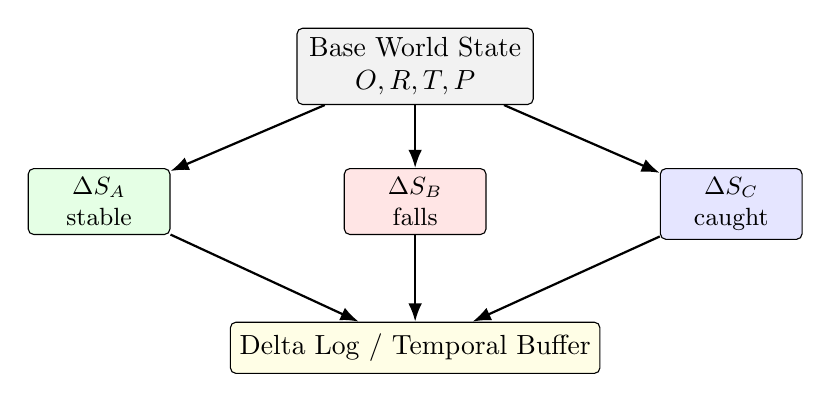
\begin{tikzpicture}[
  node distance=0.45cm,
  mem/.style={draw, rounded corners=2pt, minimum width=3.0cm, minimum height=0.65cm, align=center},
  delta/.style={draw, rounded corners=2pt, minimum width=1.8cm, minimum height=0.55cm, align=center, font=\small},
  arrow/.style={-Latex, thick}
]
\node[mem, fill=gray!10] (base) {Base World State\\$O,R,T,P$};
\node[delta, below left=0.8cm and 1.6cm of base, fill=green!10] (d1) {$\Delta S_A$\\stable};
\node[delta, below=0.8cm of base, fill=red!10] (d2) {$\Delta S_B$\\falls};
\node[delta, below right=0.8cm and 1.6cm of base, fill=blue!10] (d3) {$\Delta S_C$\\caught};
\draw[arrow] (base) -- (d1);
\draw[arrow] (base) -- (d2);
\draw[arrow] (base) -- (d3);
\node[mem, below=1.1cm of d2, fill=yellow!10] (log) {Delta Log / Temporal Buffer};
\draw[arrow] (d1) -- (log);
\draw[arrow] (d2) -- (log);
\draw[arrow] (d3) -- (log);
\end{tikzpicture}
\caption{Supplementary branch-memory schematic. A WPU shares the base state and
stores branch-specific deltas, reducing memory from \(O(BN)\) to \(O(N +
B\Delta)\) when branches are local.}
\label{fig:supp-branch-memory}
\end{figure}

\begin{table}[h]
\centering
\begin{tabular}{rrrr}
\toprule
Background objects & Sparse ratio & Hybrid ratio & Dense ratio \\
\midrule
0 & 0.0000 & 0.0000 & 1.0000 \\
20 & 0.0000 & 1.0000 & 0.0000 \\
80 & 1.0000 & 0.0000 & 0.0000 \\
\bottomrule
\end{tabular}
\caption{Supplementary routing sweep. The same local event routes differently
depending on the fraction of world state affected by the event.}
\label{tab:supp-routing}
\end{table}

\begin{table}[h]
\centering
\begin{tabular}{lccc}
\toprule
Model & Acc. at \(N=4\) & Acc. at \(N=24\) & Acc. at \(N=84\) \\
\midrule
WPU routed & 0.6719 & 0.7969 & 0.6719 \\
WPU sparse & 0.7812 & 0.8047 & 0.6719 \\
WPU hybrid & 0.7812 & 0.7969 & 0.7969 \\
WPU dense & 0.6719 & 0.6719 & 0.6719 \\
Dense graph & 0.4219 & 0.5000 & 0.5938 \\
Serialized token & 0.5625 & 0.6641 & 0.7891 \\
\bottomrule
\end{tabular}
\caption{Supplementary baseline and ablation branch accuracy after 100 training
steps. The result supports a regime hypothesis rather than universal WPU
dominance.}
\label{tab:supp-baselines}
\end{table}

\begin{table}[h]
\centering
\begin{tabular}{lcccc}
\toprule
Regime & Best WPU & Accuracy & Best non-WPU & Accuracy \\
\midrule
\(N=4\) & WPU hybrid & \(0.7242 \pm 0.0260\) & Dense graph & \(0.6398 \pm 0.1257\) \\
\(N=24\) & WPU hybrid & \(0.7320 \pm 0.0280\) & Graph Transformer & \(0.6609 \pm 0.0680\) \\
\(N=84\) & WPU hybrid & \(0.7508 \pm 0.0244\) & Graph Transformer & \(0.6953 \pm 0.0388\) \\
\(N=204\) & WPU sparse/routed & \(0.4516 \pm 0.1957\) & Graph Transformer & \(0.7172 \pm 0.0615\) \\
\bottomrule
\end{tabular}
\caption{Supplementary robust baseline comparison over five seeds, 150 training
steps, and 256 evaluation samples per condition.}
\label{tab:supp-robust-baselines}
\end{table}

\begin{table}[h]
\centering
\resizebox{\linewidth}{!}{%
\begin{tabular}{llcl}
\toprule
Change type & Measured bracket & Estimated \(N\) & Interpretation \\
\midrule
Route: dense to hybrid & \(12 \to 16\) & 16 measured & hard scheduler crosses \(\rho < 0.25\) \\
Route: hybrid to sparse & \(52 \to 68\) & 68 measured & hard scheduler crosses \(\rho < 0.05\) \\
Accuracy: WPU vs non-WPU & \(108 \to 132\) & \(\approx 120\) & WPU-family advantage disappears \\
Runtime: routed WPU vs token & \(108 \to 132\) & \(\approx 124\) & routed sparse becomes faster than token \\
Runtime: routed WPU vs dense graph & \(164 \to 204\) & \(\approx 178\) & routed sparse becomes faster than dense graph \\
\bottomrule
\end{tabular}
}
\caption{Supplementary dense \(N\)-sweep change points over
\(N=4,8,12,16,24,36,52,68,84,108,132,164,204,260\).}
\label{tab:supp-n-sweep-change}
\end{table}

\begin{figure}[h]
\centering
\begin{subfigure}{0.98\linewidth}
\centering

\includegraphics[width=0.95\linewidth]{docs/figures/n_sweep_delta.png}
\caption{Accuracy crossover curve. Positive values mean the best WPU variant
exceeds the best non-WPU baseline.}
\end{subfigure}

\begin{subfigure}{0.98\linewidth}
\centering

\includegraphics[width=0.95\linewidth]{docs/figures/n_sweep_routes.png}
\caption{Routed WPU path transition at branch pressure \(B=3\).}
\end{subfigure}
\caption{Supplementary dense \(N\)-sweep evidence. Scheduler transitions occur
near the theoretical \(\rho\) thresholds, but accuracy and runtime crossovers do
not yet align.}
\label{fig:supp-n-sweep}
\end{figure}

\begin{table}[h]
\centering
\resizebox{\linewidth}{!}{%
\begin{tabular}{rcccl}
\toprule
\(N\) & Best \(B\) & Best routed acc. & Best runtime ms/sample & Route changes \\
\midrule
24 & 1 & 0.7258 & 0.6452 & \(B=1\) sparse, \(B=2\) hybrid, \(B=6\) dense \\
84 & 1 & 0.7531 & 0.7204 & \(B=1\) sparse, \(B=5\) hybrid \\
132 & 1 & 0.6305 & 0.6050 & \(B=1\) sparse, \(B=7\) hybrid \\
204 & 1 & 0.4594 & 0.6483 & \(B=1\) sparse, \(B=11\) hybrid \\
\bottomrule
\end{tabular}
}
\caption{Supplementary dense \(B\)-sweep over \(B=1,\ldots,16\). Increasing
branch pressure moves routed WPU toward hybrid or dense execution, but accuracy
is not monotonic in \(B\).}
\label{tab:supp-b-sweep}
\end{table}

\begin{table}[h]
\centering
\resizebox{\linewidth}{!}{%
\begin{tabular}{lrrrr}
\toprule
Model & Best step & Best acc. & Acc. at 150 & Acc. at 300 \\
\midrule
WPU routed & 300 & 0.7477 & 0.6836 & 0.7477 \\
WPU sparse & 300 & 0.7477 & 0.6836 & 0.7477 \\
WPU hybrid & 100 & 0.7719 & 0.7281 & 0.7070 \\
Dense graph & 75 & 0.7617 & 0.6125 & 0.6961 \\
Graph Transformer & 75 & 0.7906 & 0.6555 & 0.7555 \\
Serialized token & 75 & 0.7875 & 0.6422 & 0.7063 \\
\bottomrule
\end{tabular}
}
\caption{Supplementary dense training-step sweep at \(N=84, B=3\). A single
fixed training budget is not sufficient evidence of model-family dominance.}
\label{tab:supp-step-sweep}
\end{table}

\begin{figure}[h]
\centering
\begin{subfigure}{0.98\linewidth}
\centering

\includegraphics[width=0.95\linewidth]{docs/figures/relation_noise_accuracy.png}
\caption{Branch accuracy under irrelevant relation noise.}
\end{subfigure}

\begin{subfigure}{0.98\linewidth}
\centering

\includegraphics[width=0.95\linewidth]{docs/figures/affected_strong_background_mse.png}
\caption{Affected-background MSE under increasing affected-region size.}
\end{subfigure}
\caption{Supplementary controlled stress tests. Relation noise tests robustness
to irrelevant edges; affected count tests whether local-update models remain
valid when the changed region becomes less local.}
\label{fig:supp-controlled-stress}
\end{figure}

\FloatBarrier


\end{document}
